\part{Expectativas}
\chapter[Conclusões]{Conclusões}

Por meio dos conteúdos apresentados, verificou-se que o projeto é viável e a até esse momento por meio de pesquisas bibliográficas percebeu-se a importância do novo prédio sustentável e inteligente para comunidade da Faculdade do Gama.O mesmo será capaz de sanar problemas já existentes na Fga.Definido o escopo e a extensão do projeto o grupo ficou satisfeito em saber que o projeto pode ser utilizado no futuro pela universidade. Dessa forma o grupo buscou desenvolver um ótimo trabalho visando a utilização do mesmo. Nos próximos pontos de controle será estabelecido com mais detalhes e mais dados de como o projeto funcionará sempre visando a viabilidade e o custo benéfico do projeto.
\section{Cronograma do Projeto}

\begin{figure}[!h]
 \centering	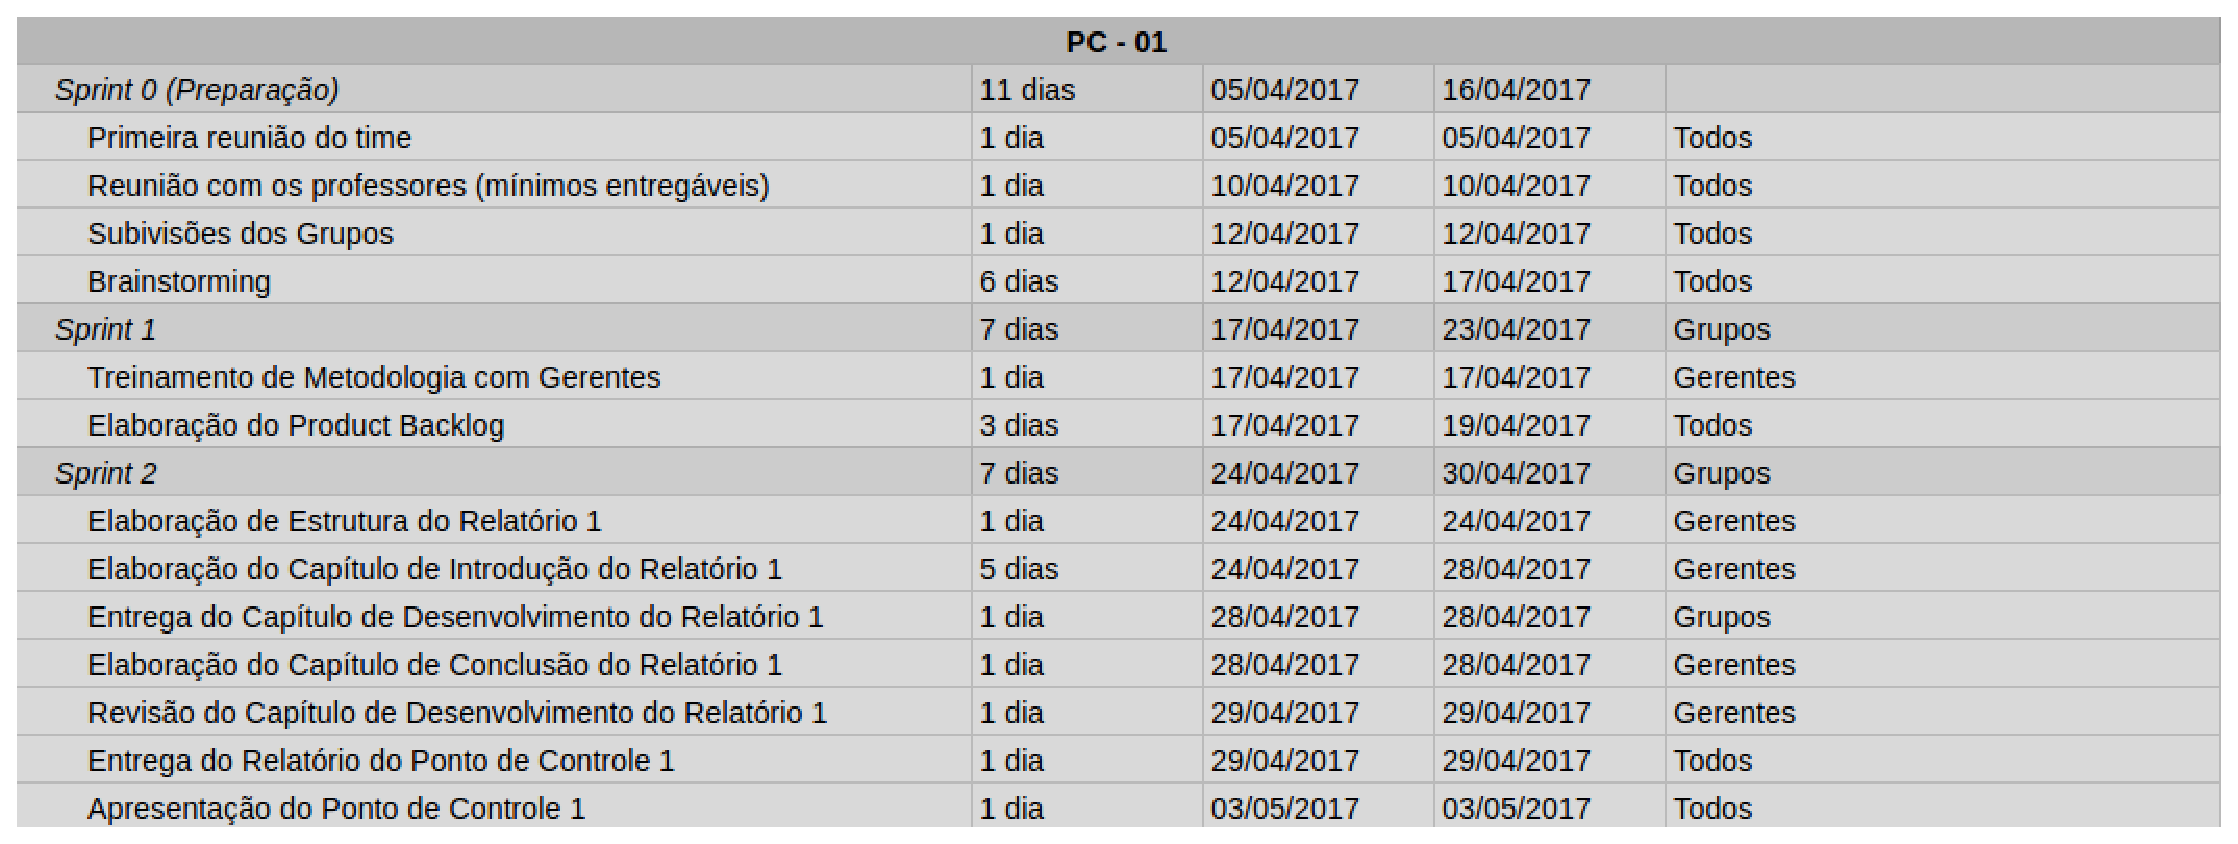
\includegraphics[keepaspectratio=true,scale=0.45]{figuras/c1.eps}
 \caption{Cronograma do Projeto - Parte 1}
 \label{fig022}
\end{figure}
\pagebreak
\begin{figure}[!h]
 \centering	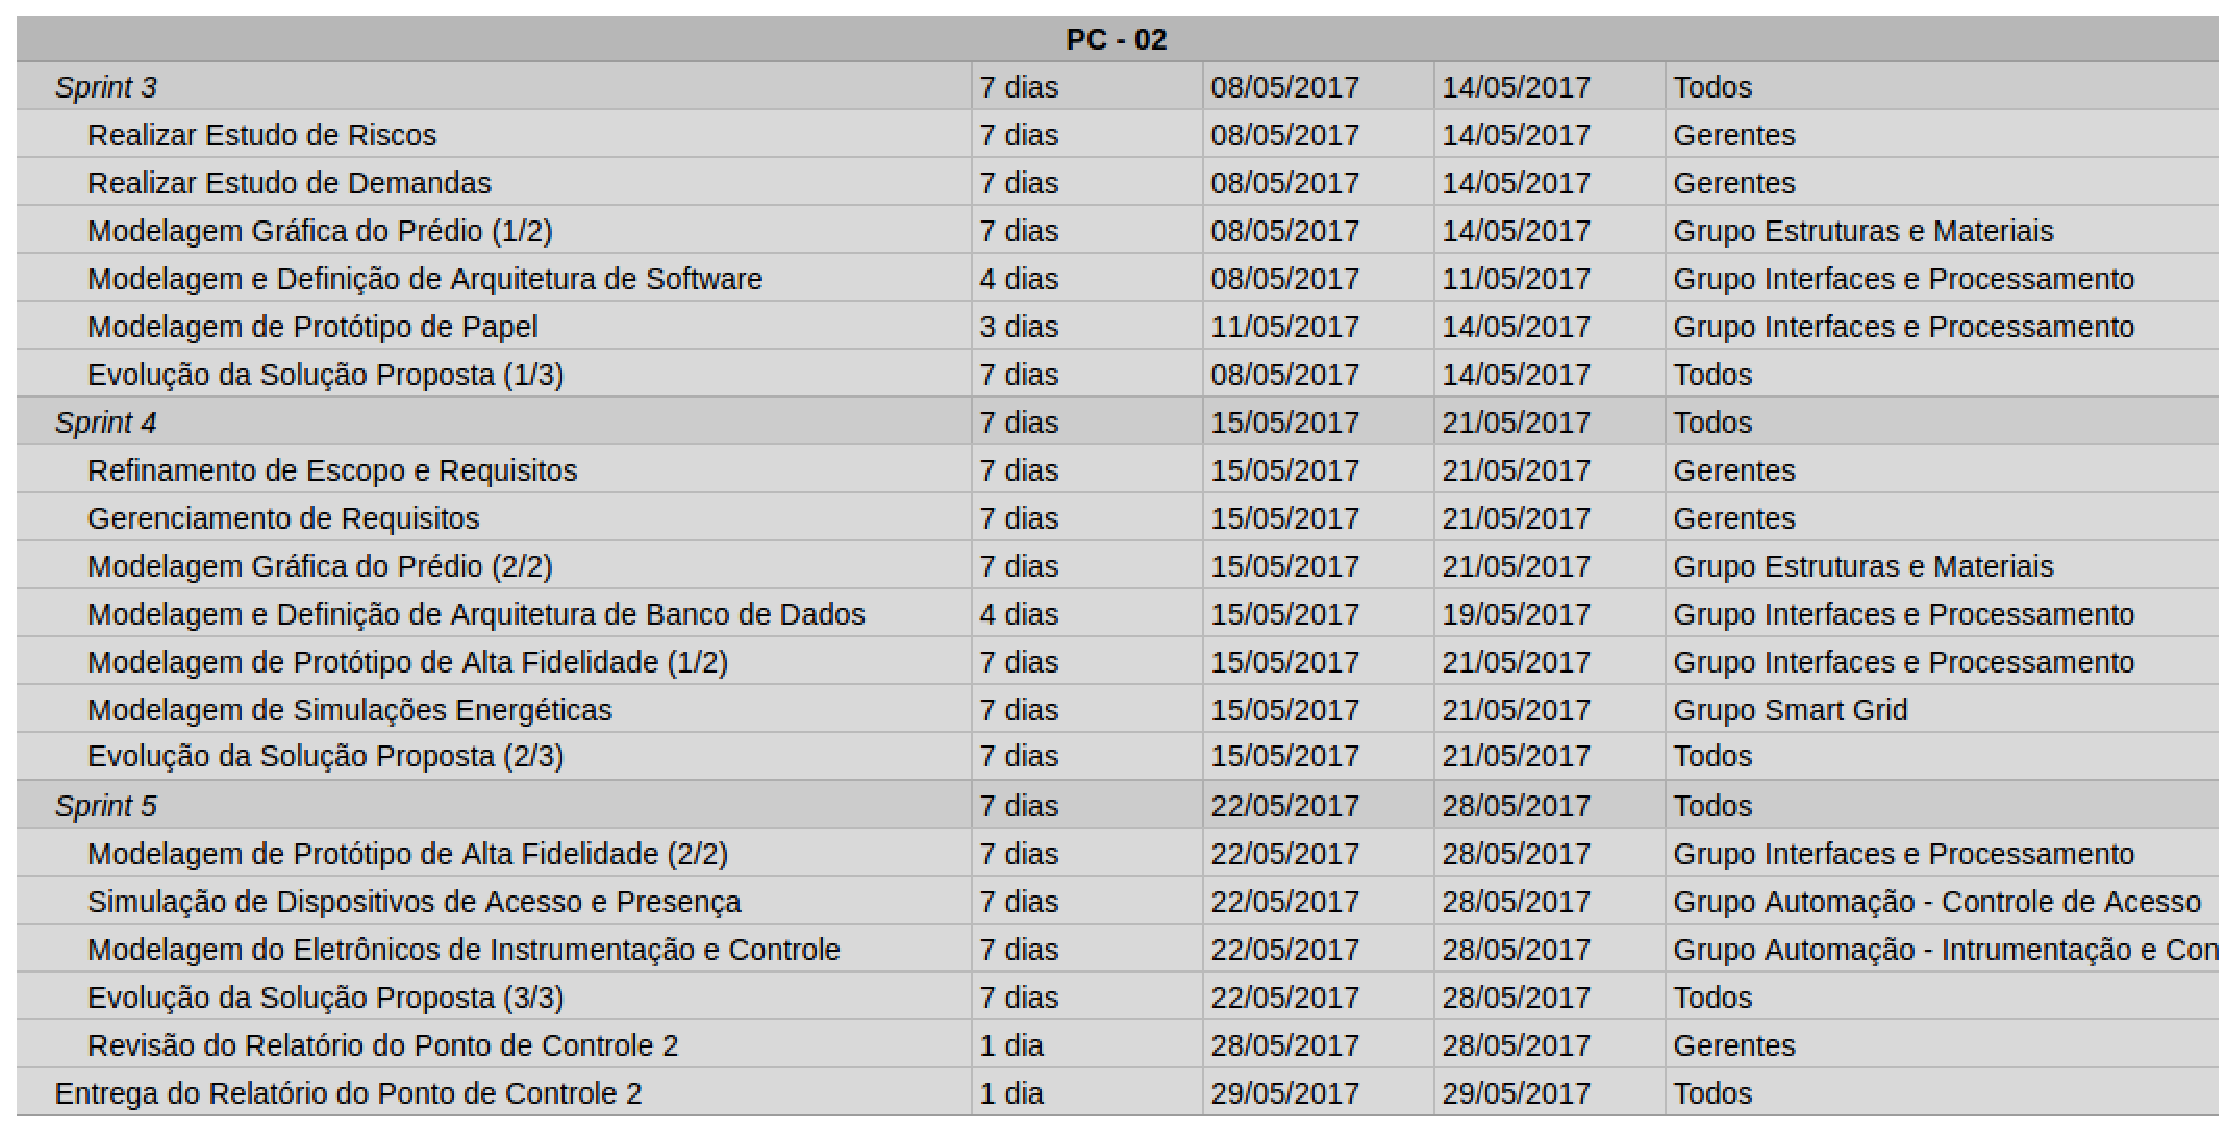
\includegraphics[keepaspectratio=true,scale=0.45]{figuras/c2.eps}
 \caption{Cronograma do Projeto - Parte 2}
 \label{fig022}
\end{figure}

\begin{figure}[!h]
 \centering	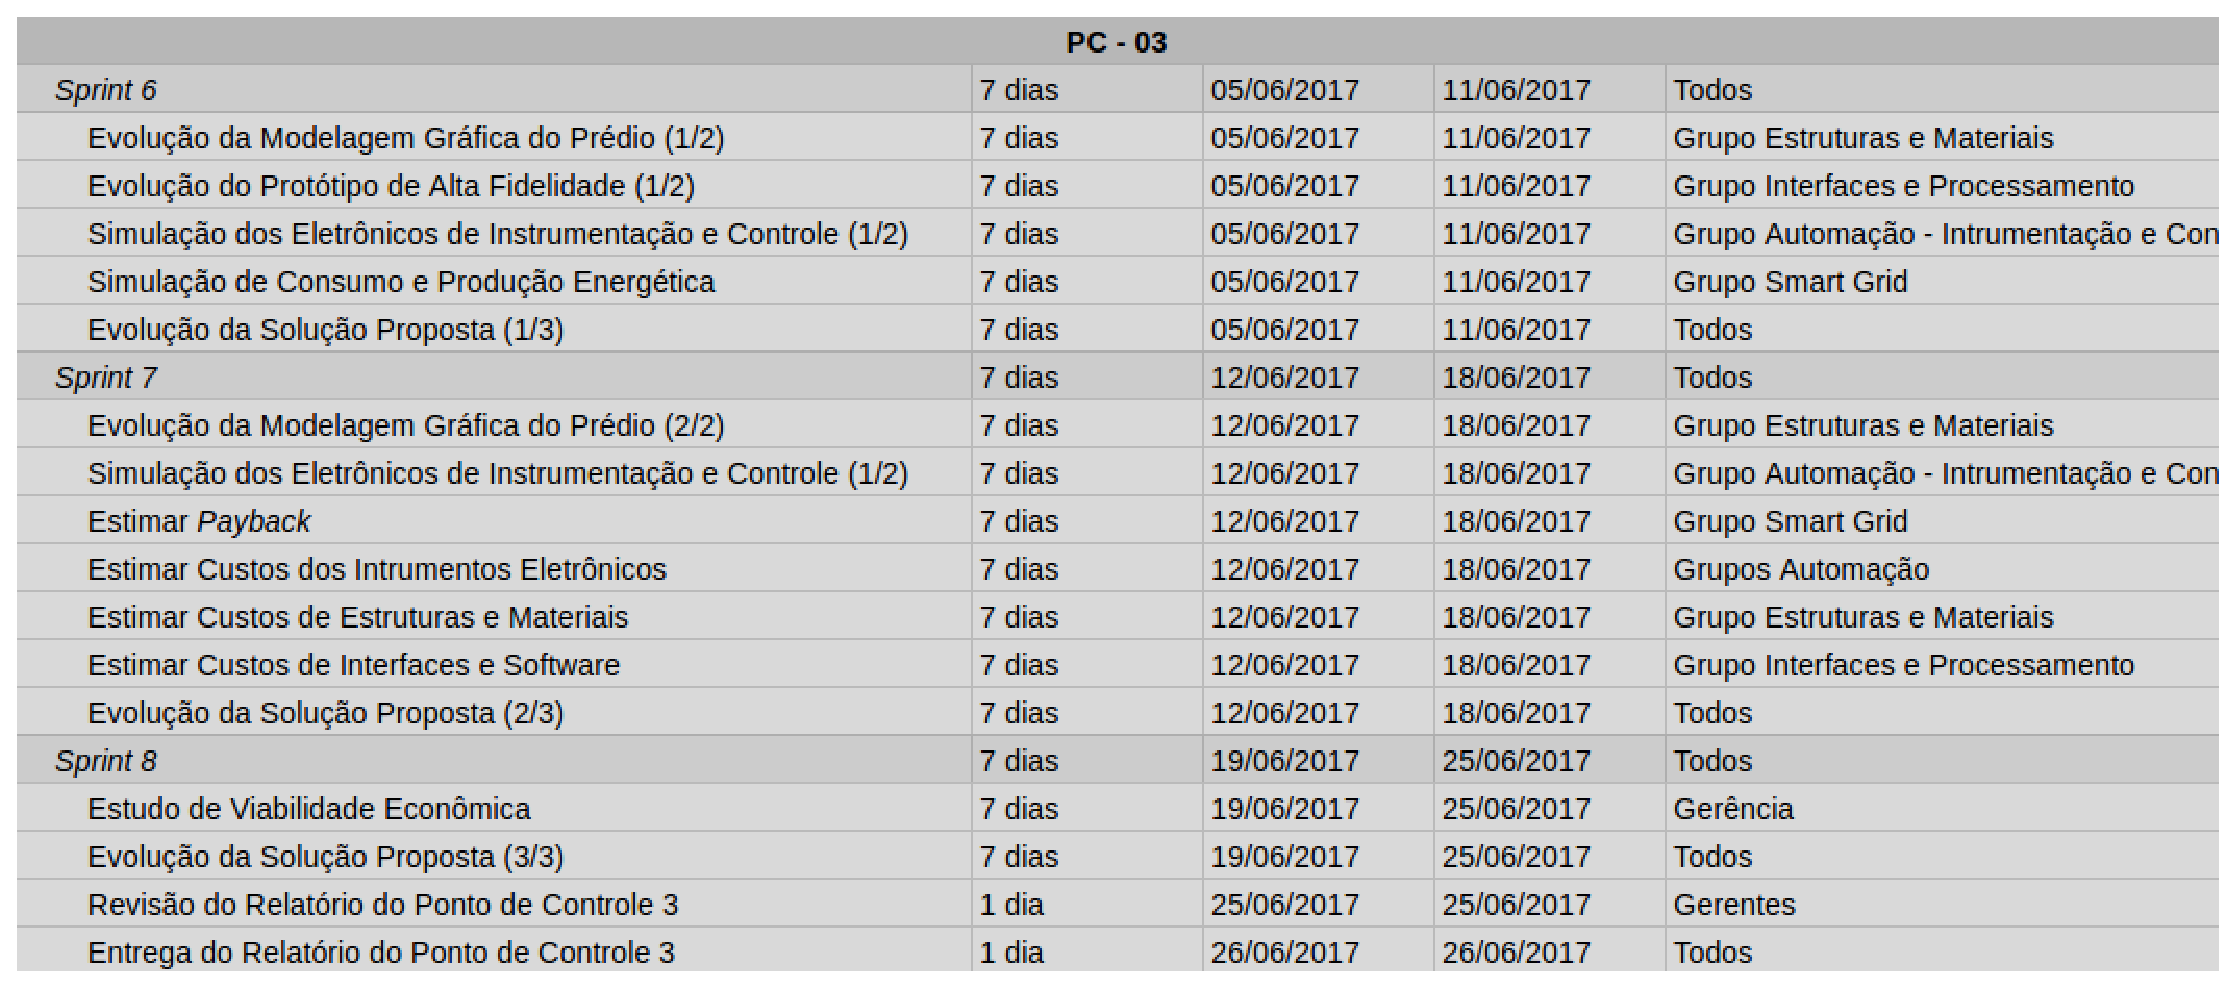
\includegraphics[keepaspectratio=true,scale=0.45]{figuras/c3.eps}
 \caption{Cronograma do Projeto - Parte 3}
 \label{fig022}
\end{figure}

\section{Próximos Pontos de Controle}

Para o próximo ponto de controle serão aprofundados os estudos dos riscos e demandas identificados no projeto. Ainda serão realizadas as representações dos sistemas usados no prédio e do prédio em si além da simulação de um dos sistemas, os dispositivos de acesso e presença.
 Para o último ponto serão feitas ainda as simulações de consumo e produção de energia, simulação dos eletrônicos de instrumentação e controle. Além disso, nesse ponto de controle o foco é mostrar a viabilidade econômica do projeto através das estimativas de payback, dos custos de cada segmento trabalhado.
